%\nocite{abc} for the books/lectures notes/articles

% all the following is to make the titlepage, but in the book format it gets screwed up
% \begin{figure}[t]
%      \centering
%      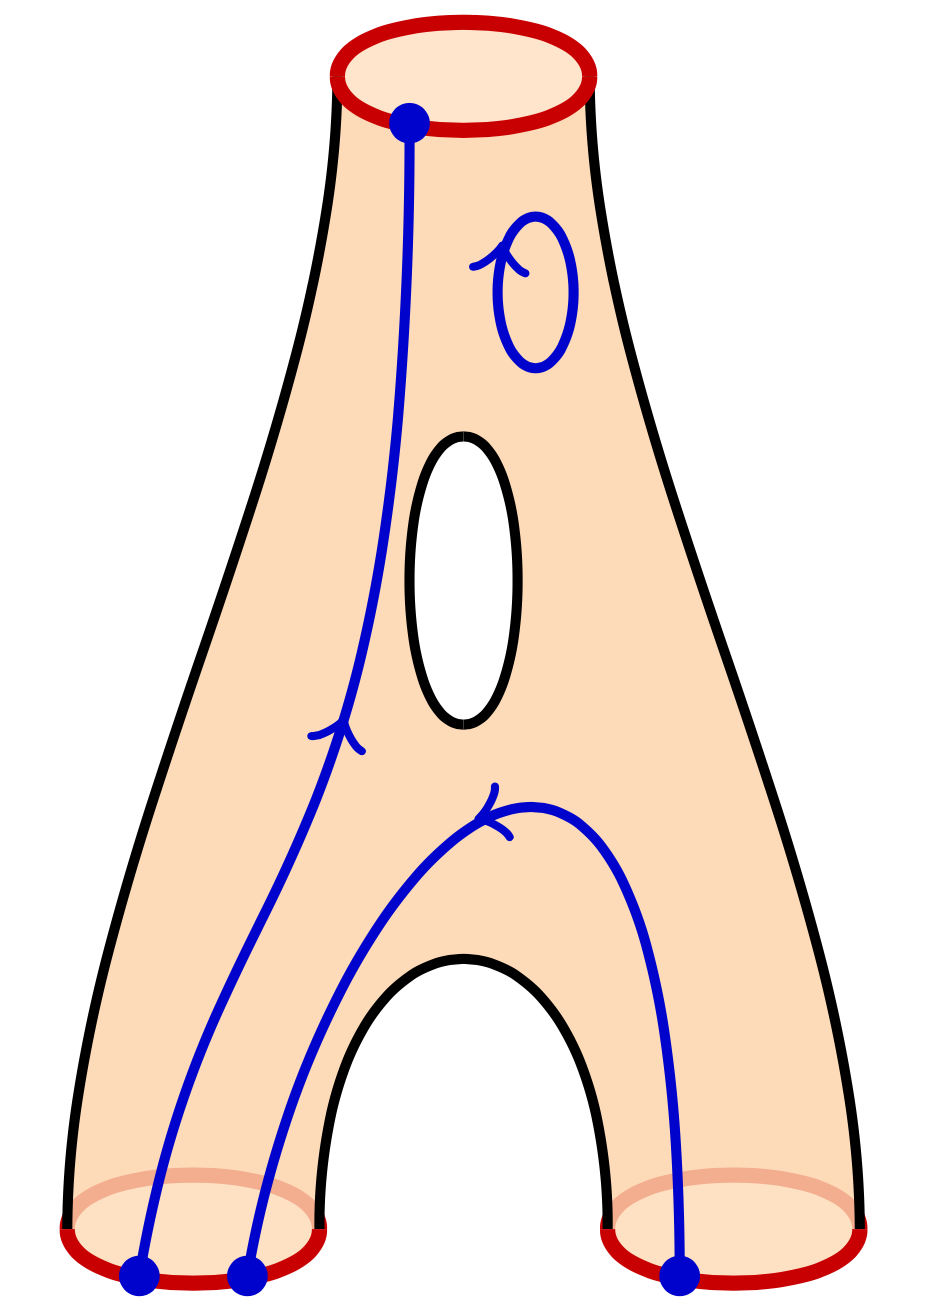
\includegraphics[width=9.50cm]{images/Lecture 1/cover.png}
%      \vspace{1mm}
%  \end{figure}
% \maketitle

% \thispagestyle{empty}

% \vspace{2mm}
% \begin{minipage}[t]{0.47\textwidth}
%    \textnormal{\large{\bf \textcolor{black}{Tutor:\\[2mm]}}}{\large \textcolor{black}{Anja \v{S}vraka}}
% \end{minipage}
% \hfill
% \begin{minipage}[t]{0.47\textwidth}\raggedleft
%    \textnormal{\large{\bf \textcolor{black}{Notes created by:\\[2mm]}}}
%    {\large \textcolor{black}{Luca Ipsale}}\\
%       {\large\textcolor{black}{William Luciani}}\\
%       {\large\textcolor{black}{Andrea Sittoni}}\\
%       {\large\textcolor{black}{Üzeyir Sa\c{c}{\i}kay}}\\
%       {\large\textcolor{black}{Jacob Skarby}}
% \end{minipage}

\pagenumbering{roman}
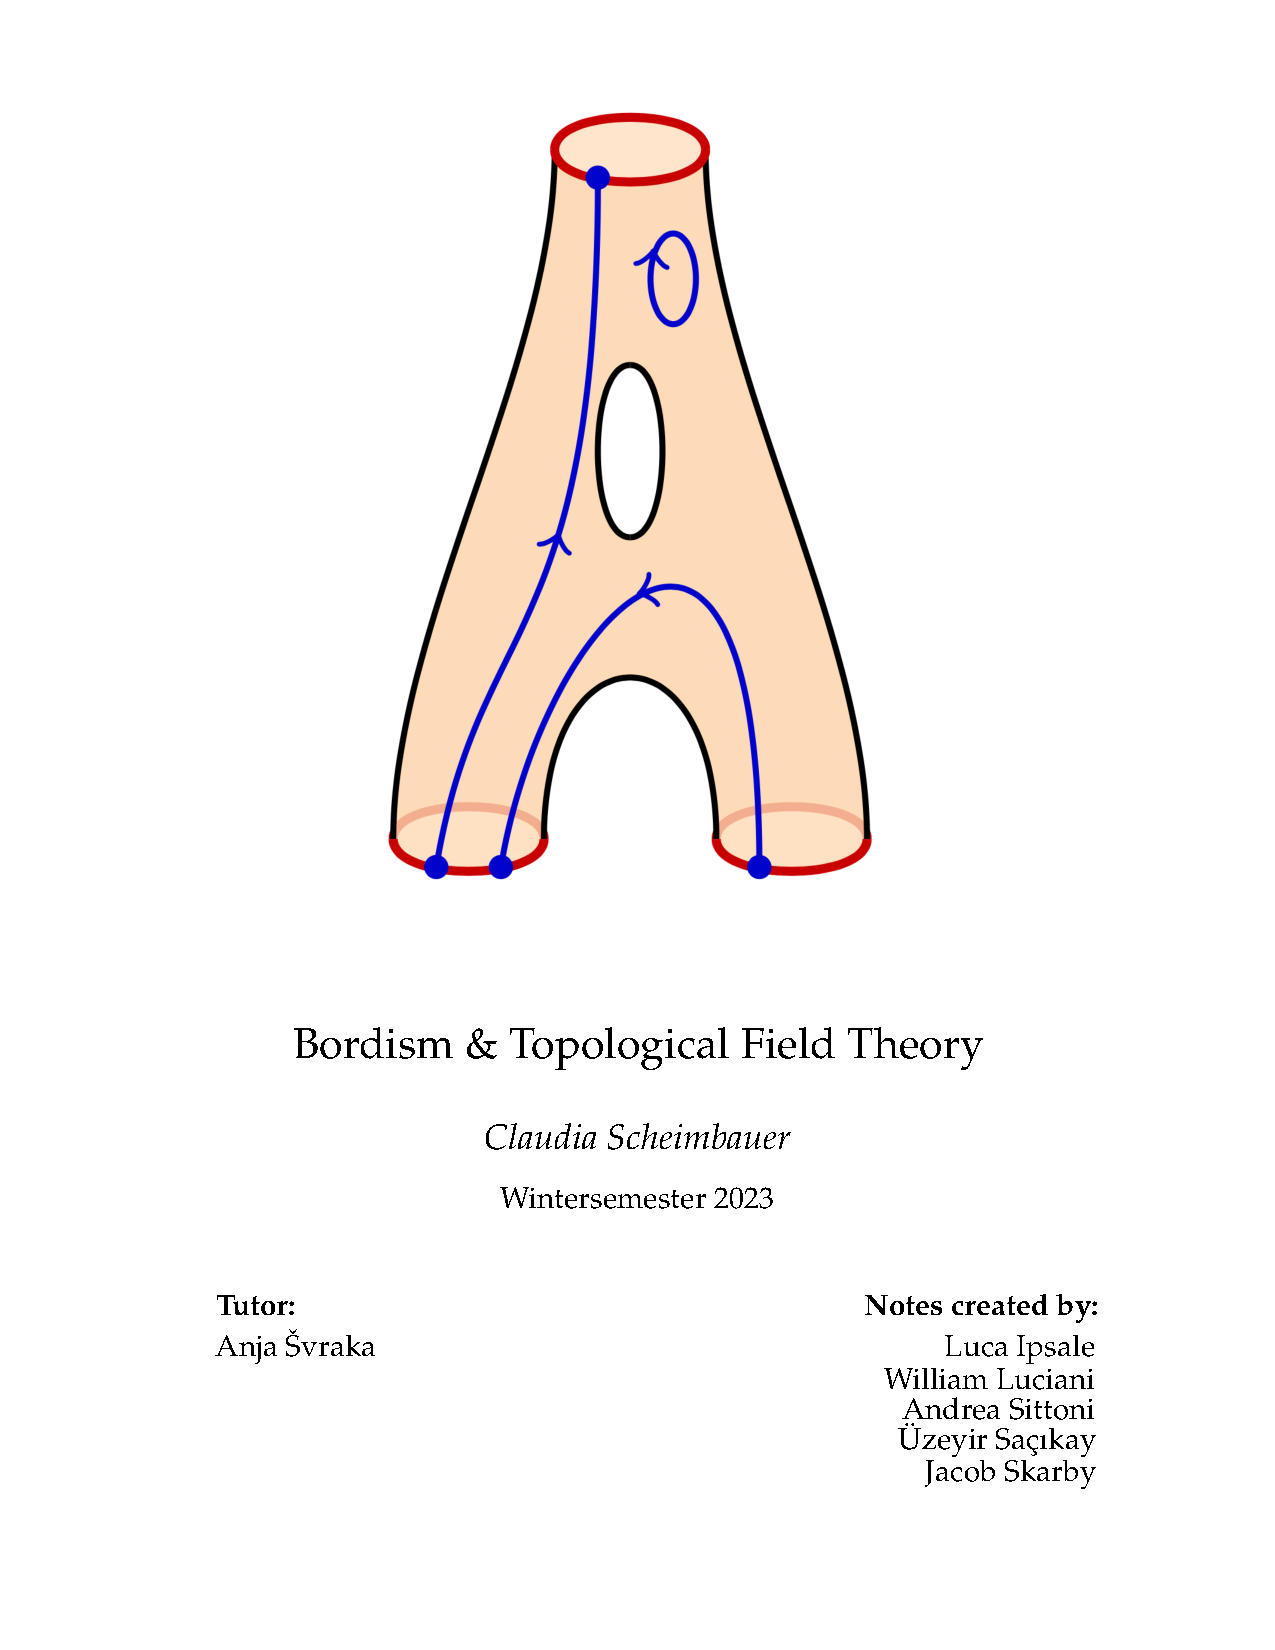
\includepdf{titlepage}

\clearpage
\thispagestyle{empty}
\cleardoublepage

\clearpage
\thispagestyle{empty}
\begin{flushright}
\null\vspace{\stretch{1}}
\textit{The mathematical facts worthy of being studied\\
are those which, by their analogy with other facts,\\
are capable of leading us to the knowledge of a mathematical law\\
just as experimental facts lead us to the knowledge of a physical law.\\
They reveal the kinship between other facts, long known,\\
but wrongly believed to be strangers to one another.\\
\hfill\break
$-$H. Poincaré}\\
\vspace{\stretch{2}}\null
\end{flushright}
\clearpage

\chapter*{\huge{\textcolor{black}{For the reader}}}
\hfill
\vspace{0.50cm}\\
These are the lecture notes of the course \textit{``Bordism and Topological Field Theory''} held by Prof.\hspace{1mm}Dr. Claudia Scheimbauer (\href{mailto:scheimbauer@ma.tum.de}{scheimbauer@ma.tum.de}) during the Wintersemester 2023/2024 at the \textit{Technische Universität München}. The tutorial sessions are held by Anja \v{S}vraka (\href{mailto:svr@ma.tum.de}{svr@ma.tum.de}).\hspace{1.5mm}The notes are typed by Luca Ipsale (\href{mailto:luca.ipsale@campus.lmu.de}{luca.ipsale@campus.lmu.de}), William Luciani (\href{mailto:w.luciani@campus.lmu.de}{w.luciani@campus.lmu.de}), Andrea Sittoni (\href{mailto:sittoniandrea@gmail.com}{sittoniandrea@gmail.com}) and Üzeyir Sa\c{c}{\i}kay (\href{mailto:uzeyirsacikay@gmail.com}{uzeyirsacikay@gmail.com}). Exercises are also implemented in the notes by Jacob Skarby (\href{mailto:jacob.skarby@tum.de}{jacob.skarby@tum.de}). If you find
 errors or have suggestions of any kind, please write us an e-mail.

\vspace{1cm}

{\LARGE \warning These notes have not been proofread by Prof. Scheimbauer, use at your own risk}.

\updateinfo
\thispagestyle{empty}



\clearpage
\thispagestyle{empty}
\cleardoublepage
\section*{Notational Conventions}
\begin{notat}
    Throughout these notes we will abuse notation indicating a collection with some structure on it just by
     writing down the collection, e.g. denoting a monoid $(M,\cdot)$ by $M$, a metric space $(X,d)$ by
      $X$ etc...
\end{notat}
\begin{notat}
    By '$n$-manifold' and '$n$-bordism', we mean respectively a manifold of dimension $n$
     and bordism a bordism of dimension $n$.
\end{notat}
\begin{notat}
    We often denote equivalence classes just with a representative thereof. 
\end{notat}

\begin{notat}[\extra]
    We use the symbol '\extra' at the end of titles of sections, definitions or theorems that depart from the
    content of the class and deepen some aspects of topics we did not cover in the lectures.
    
    They are often sketchy. Their aim is to convey the intuition behind exciting topics in the field of TFTs
     or neighouring ones (and often
    convince you that $\infty$-categories are cool and useful\footnote{Regarding this, we are very 
    happy and excited to communicate that the next semester (SoSe2024) there will be a seminar
    regarding simplicial homotopy theory and $\infty$-categories at LMU. If you are interested or 
    have any questions regarding this, contact Prof. Land
     (\href{mailto:Markus.land@math.lmu.de}{Markus.land@math.lmu.de}) and check
     \href{https://www.markus-land.de}{his website}.}). They have been written by Andrea Sittoni.
    Please send corrections, suggestions and comments.
\end{notat}
In this kind of sections we have the following conventions.
\begin{notat}
We denote the $(\infty,1)$-category of spaces/$\infty$-groupoids both with $\mathscr{S}$,
 $\operatorname{Grpd}_\infty$ and with $\infty\operatorname{-Grpd}$. $\mathscr{S}$ stands for 
 $\mathscr{S}$paces. This is motivated by the
  homotopy hypothesis, see \ref{HomotopyHypothesis}.
\end{notat}
\begin{notat}
When there is no ambiguity, we denote $(\infty,1)$-categories as $\infty$-categories. We denote the
$(\infty,2)$-category of all $(\infty,1)$-categories with $\Cat_\infty$ or $\infty$-Cat.
\end{notat}
\section*{Prerequisites}
The notes strive to be as self-contained as possible. We do assume however knowledge of linear algebra,
basic notions from analysis, e.g. smoothness, and basic notions of topology, e.g. 
paracompactness. Knowledge of algebraic topology is helpful but not necessary to understand the
most important parts.
\section*{Acknowledgements}
Apart from Prof. Scheimbauer's lectures and the cited references,
we often got inspiration from the nLab (\url{https://ncatlab.org/nlab/show/HomePage}) and from notes
on algebraic topology by Prof. Land (available on \url{https://www.mathematik.uni-muenchen.de/~gritscha/TOP1-23.php}).

\thispagestyle{empty}
\hfill
\vspace{0.50cm}
\textcolor{black}{\tableofcontents}